\subsection{Micro-Doppler}
The concept of micro-Doppler was first proposed by Chen in 2000 \cite{tahmoush2009remote}. Micro-Doppler signatures reflect the periodic kinetic characteristics of a moving object. Modulations of the radar resulted from the arms, the legs and even the body sway have been investigated by researchers \cite{ram2008simulation,tahmoush2009radar,zhang2007acoustic}. 

Given an electromagnetic wave transmitted by an RF radar, the frequency of the received signals due to a moving target with a constant radial velocity $v$ with respect to the radar is:
\begin{equation}
f=f_0 (1+2v/c),
\end{equation}
where $f_0$ is the carrier frequency of the radar and  $c$ is the speed of the light. The Doppler frequency shift due to the target is:
\begin{equation}
f_D=f_0  (2v/c),
\end{equation}
which is proportional to the velocity of the target relative to the radar.

In the case of an articulated body such as a walking person, the torso, each arm and each leg has its own velocity, and even when the torso's velocity is constant, the velocity of the limbs changes over time \cite{zhang2007acoustic}. The Doppler signature $f_{Dsig}$ for such a complex object has multiple time-dependent frequency shifted components and it is defined as:
\begin{equation}
f_{Dsig} (t)=f_0\sum_{i=1}^{N}2v_i (t)/c,
\end{equation}
where $N$ is the number of parts of the moving target, $v_i (t)$ is the velocity of each part as a function of the time. The analytic signal of the returned echo from such a target is given by: 
\begin{equation}
\hat{S}_R (t)=e^{j2 \pi f_0 t} e^{j2\pi f_{Dsig} (t)t},
\end{equation}
The combination of the received signal $\hat{S}_R (t)$ with the transmitted signal $\hat{S}_T (t)$ as follows:
\begin{equation}
\hat{S}_R (t) 〖\hat{S}_T ̂(t)〗^*=e^{j2\pi f_0 t},
\end{equation}
allows the extraction of the Doppler signature from the data. This is the component of the signal that contains the micro-Doppler information of the target and it can be used for target or activity recognition and classification. The bandwidth of the resulting signal is normally much smaller than the carrier frequency,  because the micro-Doppler information relies on the lower frequencies \cite{balleri2011classification}. The micro-Doppler signature can be represented in a two-dimensional time-frequency space using a Short Time Fourier Transform (STFT):  
\begin{equation}
\begin{split}
STFT(i,K)=&\sum_{n=0}^{N-1} x_i (n) e^{-j2\pi(nK/N) },\\& K=0,\ldots ,N-1
\end{split}
\end{equation}
where $x_i (n)$ is the sliding window with a given length $N$. The $i$th window is defined as:
\begin{equation}
x_i (n)=\hat{S}_R (n+i(N/2))w(n),
\end{equation}
where $w(n)$ is a weighting function.

The frequency resolution can be approximated as the inverse of the duration of the window:
\begin{equation}
T_w=N/f_s,
\end{equation}
where $f_s$ is the sampling rate, and therefore only Doppler shifts that are greater than $1/T_w$, corresponding to velocities
\begin{equation}\label{eq:ddf}
v>c/〖2f_o T〗_w,
\end{equation}
will be clearly visible \cite{balleri2011classification}. From Eq. (\ref{eq:ddf}), it can be shown that radars that work in higher frequencies have the additional advantage to induce a wider micro-Doppler bandwidth where small movements are more easily detected for a given frequency resolution, because the carrier frequency is higher \cite{balleri2011classification}.

In this paper, an STFT has been used to generate time-frequency spectrograms. Fig. \ref{fig_tf0} shows a spectrogram of the radar signals of a human walking indoors that were collected in this research. The spectrogram shows the evident periodic characteristics of a human activity. The fluctuations resulted by the limbs are attached to the main Doppler frequency resulted by the torso. 
\begin{figure}[!t]
\centering
%\captionsetup{justification=centering}
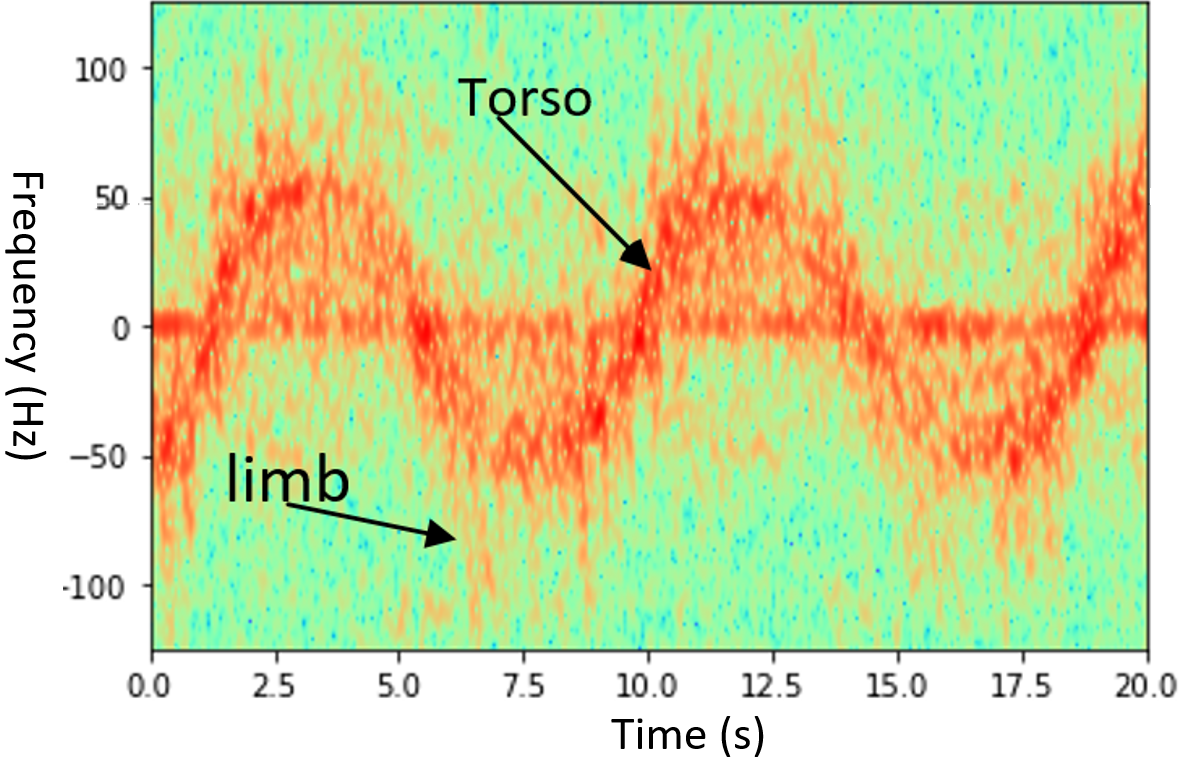
\includegraphics[width=3in]{time_frequency}
\centering
\caption{A time-frequency spectrogram of indoor human walking}
\label{fig_tf0}
\end{figure}

\subsection{The Low-power Radar System}
The Doppler radar system built in this research consists of two BumbleBee radars from Samraksh \cite{bumblebee}. The Bumblebee radar is a low-power Pulsed Doppler Radar that is designed for a variety of Wireless Sensor Network (WSN) applications. Its center frequency is 5.8 GHz; and its detection range is up to 8 meters outdoors. Unlike traditional radars, the BumbleBee is designed to be compatible at a system level with small, battery powered nodes. It only consumes about 12 mA, so when using typical 1.5v AA alkaline batteries with a capacity of 2400 mA, it can run at 100\% duty cycle for about 8 days. Each BumbleBee radar outputs data on two channels providing the in-phase  ($I$) and quadrature-phase ($Q$) signal components, which are used to form the complex signal $C=I+jQ$. The $I/Q$ output data of the BumbleBee radar represents the peak of the matched filtered data acquired for each pulse. Thus, the time interval between each data packet corresponds to the pulse repetition interval (PRI) of the radar.

Each BumbleBee radar was connected to one TelosB mote \cite{polastre2005telos} and another TelosB mote was used as a base station connected to a PC (see Fig. \ref{fig_radar}). The TelosB mote provides radio communication at low-power consumption (IEEE 802.15.4).  It has a long battery life and it is able to wake up fast from a sleep state. It is fully compatible with the open-source TinyOS, an operating system that supports large-scale, self-assembling sensor networks.
\begin{figure}[!t]
\centering
%\captionsetup{justification=centering}
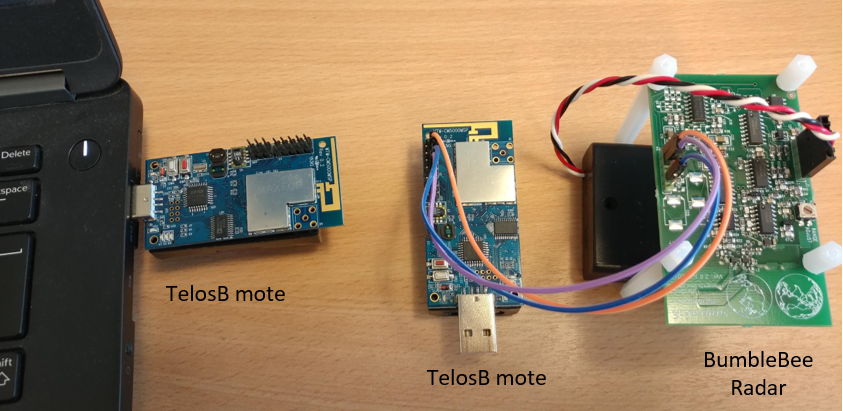
\includegraphics[width=3in]{radar}
\centering
\caption{BumbleBee radar and TelosB mote}
\label{fig_radar}
\end{figure}

In our investigation, a multi-radar system composed of two radars was used. The reason for that is because a multi-radar system collects signals of human activity from multiple angles, this provides more information for the classifiers. However, it also means more data is required to be transferred concurrently, consequently packet loss in data transmission increases in detriment to the gains in information gathering. We found that for a system set up with one base station and two radars there was an increased gain in information gathering without loss in data transmission, but for a higher number of radars the transmission data loss was noticeable.

For validating the setup of our BumbleBee radars, a corner reflector was used as a target. The corner reflector was tied to a string and hanged from the ceiling of a laboratory and pushed slightly to swing back and forth.  Our experiment followed the same set up as the corner reflector experiment presented in \cite{cagliyan2014human} that also used BumbleBee radars. The corner reflector`’s swinging was measured by the Bumblebee radars, and the collected signals were used to generate a frequency spectrogram to show the fluctuations of the reflected micro-Doppler signals. Fig. \ref{fig_validation}(a) presents the frequency spectrogram shown in \cite{cagliyan2014human} and Fig. \ref{fig_validation}(b) shows the spectrogram obtained from our radars. Both spectrograms show similar periodical fluctuations caused by the swinging of the corner reflector. In both, when the range of the swing angle declines, the amplitude of fluctuations decreases. Therefore, the setup of our Bumblebee radars was successfully validated.
\begin{figure}[!t]
\centering
%\captionsetup{justification=centering}
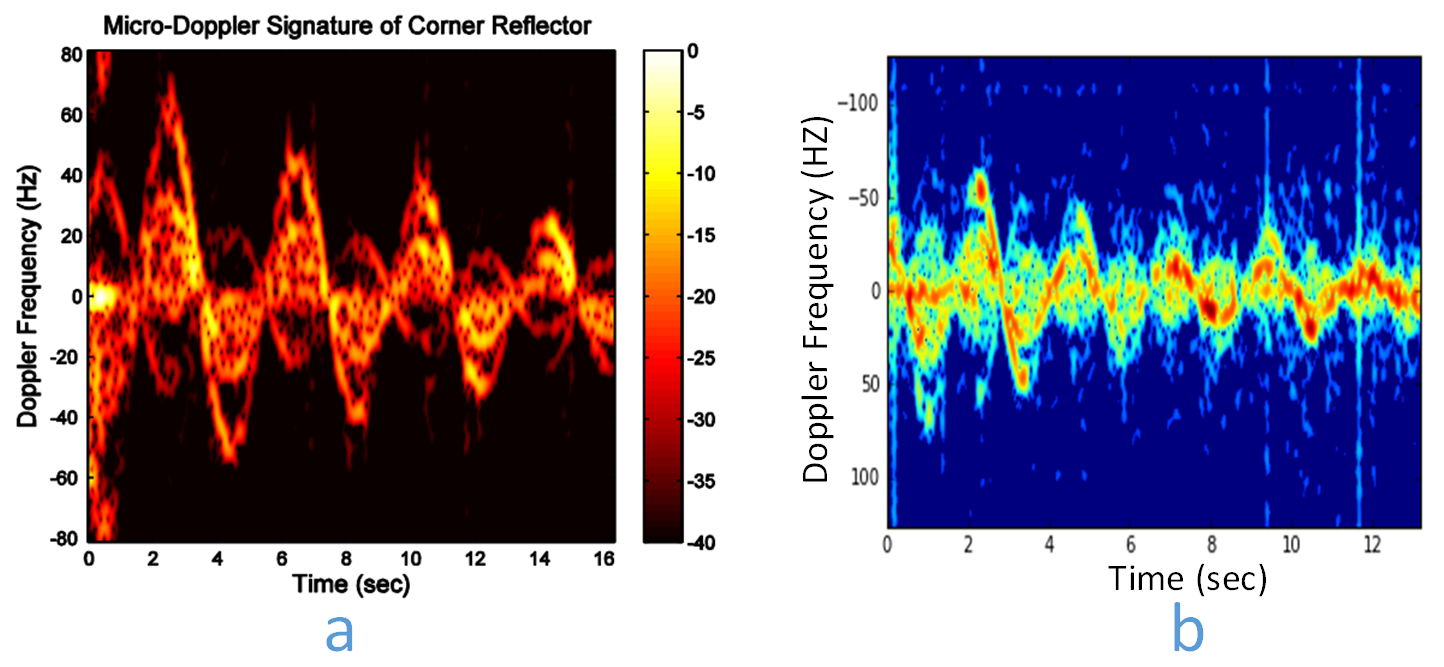
\includegraphics[width=3.5in]{validation}
\centering
\caption{Micro-Doppler signatures of a swinging corner reflector}
\label{fig_validation}
\end{figure}

The Doppler radar system was implemented outdoors. As shown in Fig.  \ref{fig_rs}, two radars (BumbleBee 1, BumbleBee 2) were placed in a straight line, eight meters apart and opposite to each other. One radar was called the \textit{primary node} (BumbleBee 1), the other was called the \textit{secondary node} (BumbleBee 2). There was a \textit{base station} (Telosb 03) connected to a laptop. The base station received data from the two Telosb motes (Telosb 01 and Telosb 02). Each mote was connected to one BumbleBee radar. The light red and light blue shadowed areas were the detection ranges of BumbleBee 1 and BumbleBee 2 respectively. The cross width of the detection ranges was from 10m to 12m. Only targets inside the detection ranges could be observed. It can be noticed that the union of two radars’ detection ranges was split into three non-overlapping ranges, which were 1-3m, 3-5m, and 5-7m relative to the primary node. The experiments were made in these three different ranges in order to tag the range labels to the micro-Doppler signatures, which were used for coarse-grained localization. The arrows represent the target movement direction relative to the radar beam. In order to investigate the effects of the angle between the direction of movement and the radar, three different directions (\ang{0}, \ang{45}, and \ang{90}) were considered. The direction of the target movements at \ang{45} was the same as at \ang{90}, however the radar beams of the primary and secondary nodes were changed to \ang{45} when performing the experiments for the \ang{45} angle.
\begin{figure}[!t]
\centering
%\captionsetup{justification=centering}
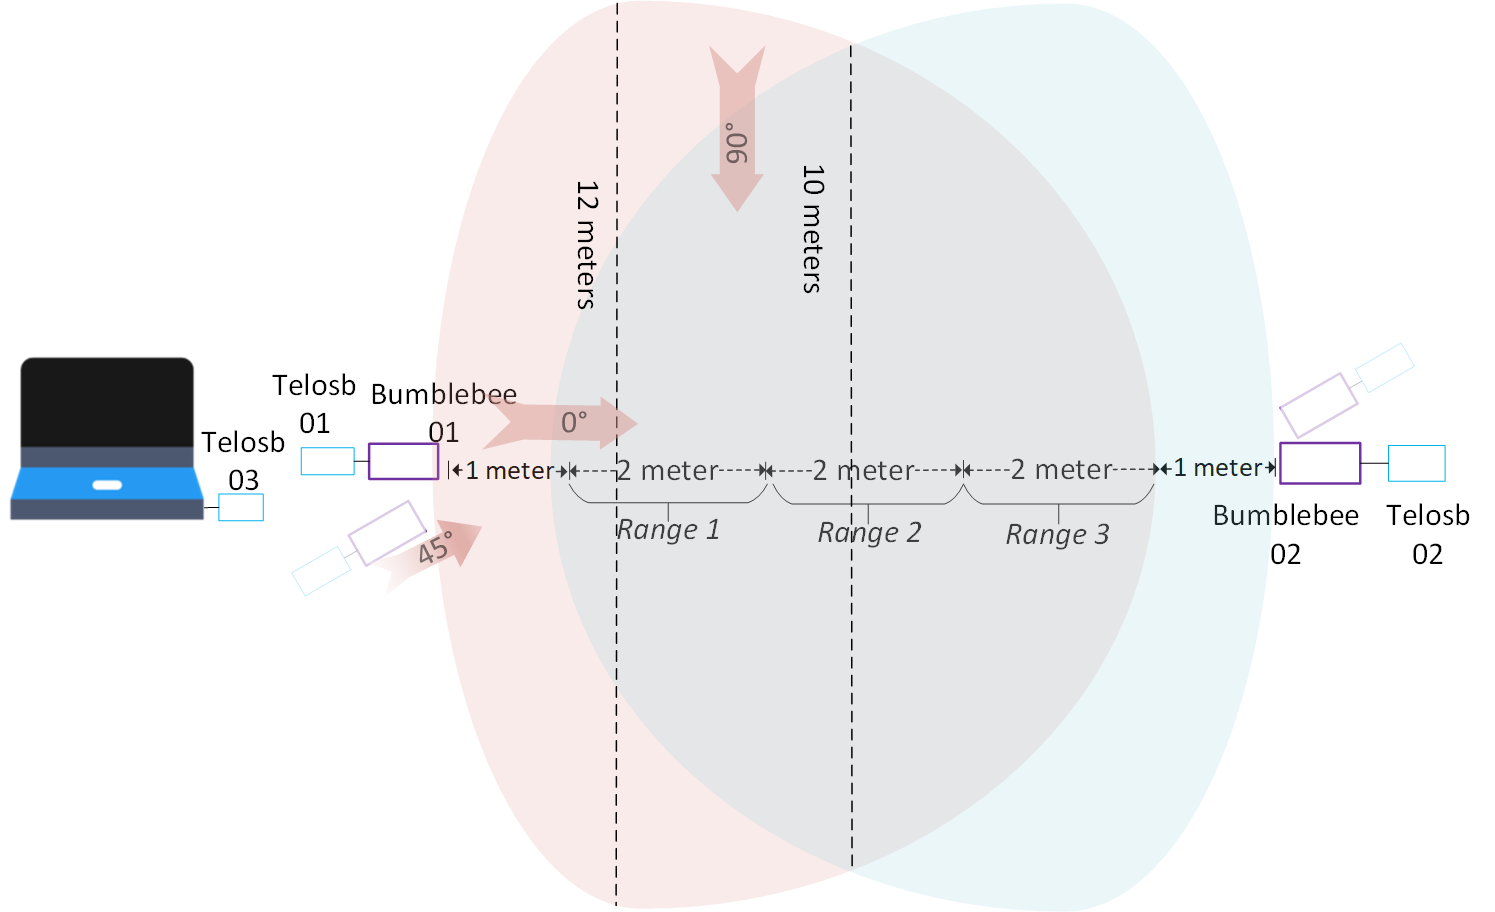
\includegraphics[width=3.6in]{radar_system}
\caption{Doppler radar system implemented in outdoors}
\label{fig_rs}
\end{figure}